\afterpage{%
    \begin{savenotes}%
        \begin{figure}[H]
            \begin{enumerate}
                \item[(a)] 
\includegraphics[scale=0.99]{plot_rank_similarity_papertop.pdf}\\
                \vspace*{-0.2cm}%
                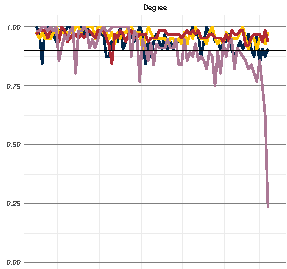
\includegraphics[scale=0.99]{plot_rank_similarity_paper_degree.pdf}\hspace*{0.1mm}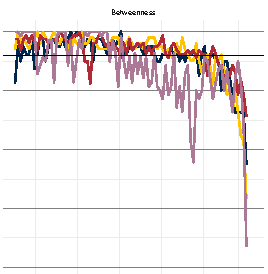
\includegraphics[scale=0.99]{plot_rank_similarity_paper_betweenness.pdf}\hspace*{-0.4mm}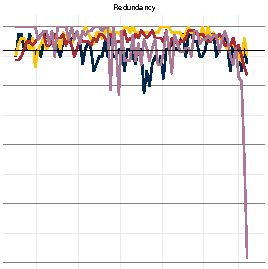
\includegraphics[scale=0.99]{plot_rank_similarity_paper_redundancy.pdf}\\
                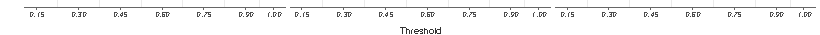
\includegraphics[scale=0.99]{plot_rank_similarity_paperbottom.pdf}
                \vspace*{-0.7cm}
                \item[(b)] \hspace*{-0.25cm}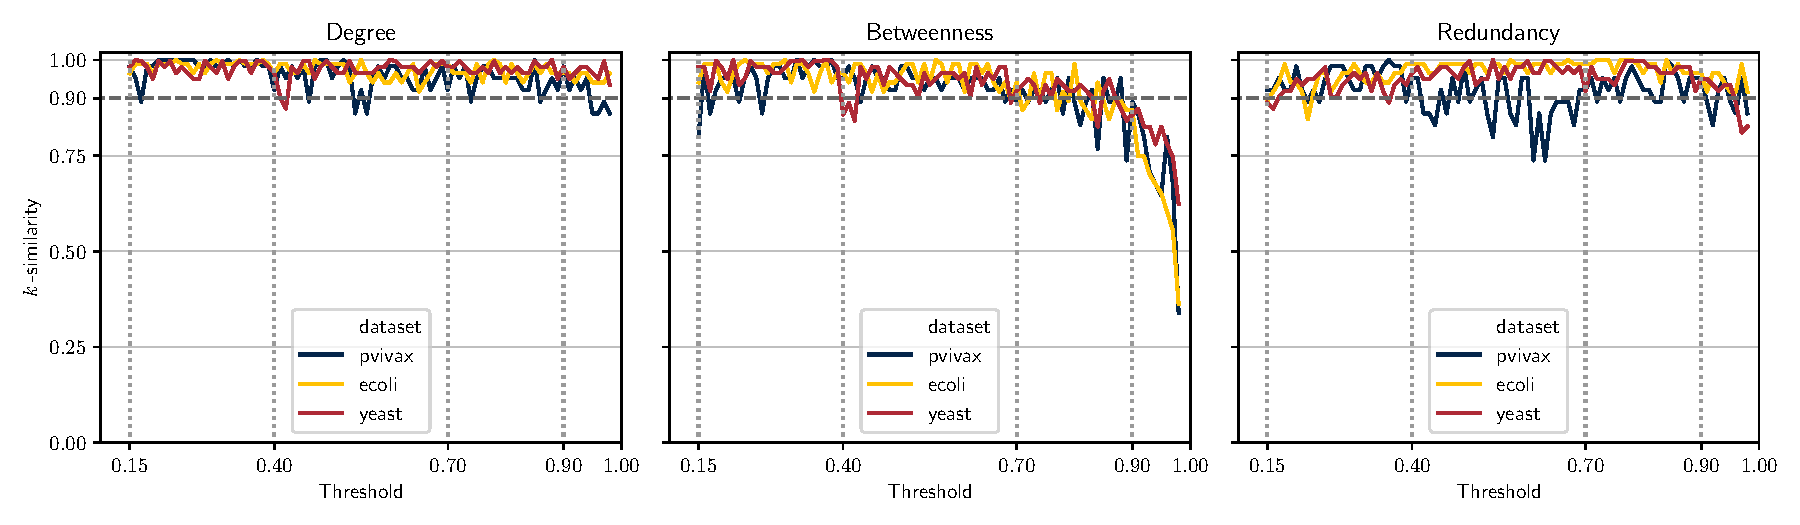
\includegraphics[align=t,width=0.96\linewidth]{plot_rank_similarity_graffs.pdf}
            \end{enumerate}
            \vspace{-0.4cm}
            \caption{$k$-similarity plots between ranks of graphs derived from protein networks\cref{foot:hpred} at consecutive thresholds, taking results from The Paper~(a) and \graffs~(b).\cref{foot:similarity_coefficients}}
            \label{fig:plot_rank_similarity}
            \vspace{0.4cm}
%\footnotetext{\label{foot:similarity_coefficients}Chosen according to \url{https://github.com/lbozhilova/measuring_rank_robustness/blob/master/figure_generation.R#L28}}
            \begin{enumerate}
                \item[(a)] 
\includegraphics[scale=0.99]{plot_relaxed_similarity_papertop.pdf}\\
                \vspace*{-0.2cm}%
                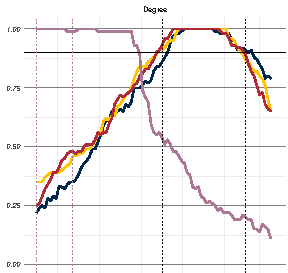
\includegraphics[scale=0.99,trim={0 0.8mm 0 0},clip]{plot_relaxed_similarity_paper_degree.pdf}\hspace*{0.2mm}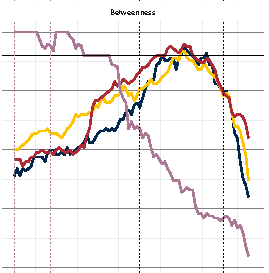
\includegraphics[scale=0.99,trim={0 0.3mm 0 0},clip]{plot_relaxed_similarity_paper_betweenness.pdf}\hspace*{-0.45mm}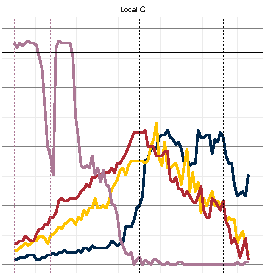
\includegraphics[scale=0.99,trim={0 0.8mm 0 0},clip]{plot_relaxed_similarity_paper_localc.pdf}\\
                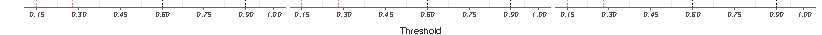
\includegraphics[scale=0.99]{plot_relaxed_similarity_paperbottom.pdf}
                \vspace*{-0.7cm}
                \item[(b)] \hspace*{-0.25cm}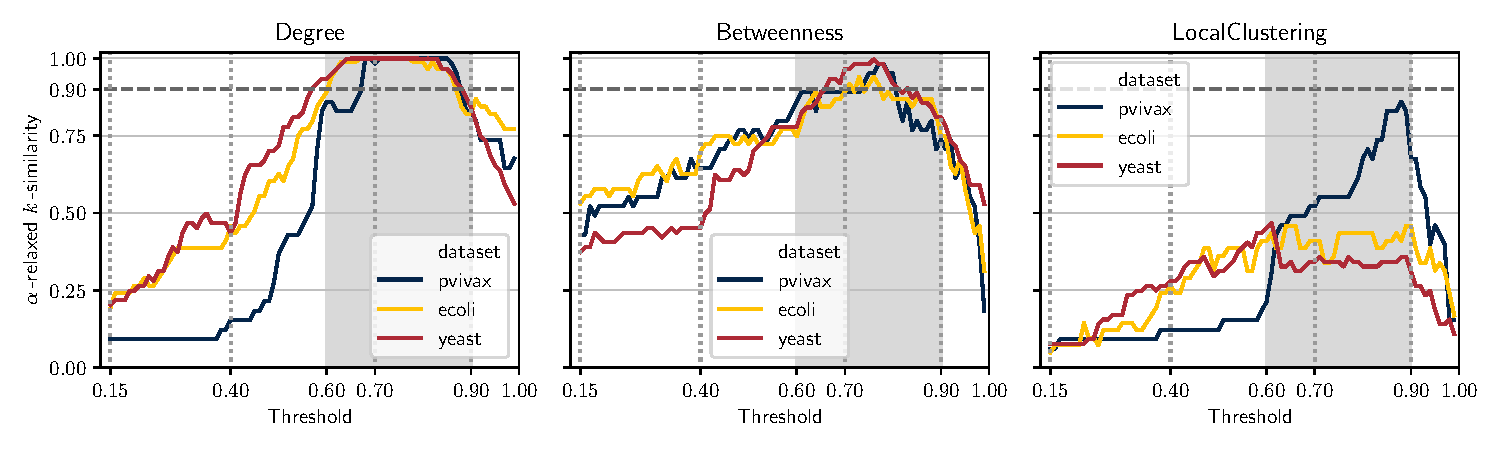
\includegraphics[align=t,width=0.96\linewidth]{plot_relaxed_similarity_graffs.pdf}
            \end{enumerate}
            \vspace{-0.4cm}
            \caption{$\alpha$-relaxed $k$-similarity plots between overall rank and ranks at individual thresholds, taking results from The Paper~(a) and \graffs~(b) on protein networks\protect\footnote{\label{foot:hpred}The HPRED dataset is not used in this dissertation and so is irrelevant}.
            The overall rank for each of 3 metrics was calculated within the ``wide medium-high confidence region'' $\left[ 0.6, 0.9 \right]$.\protect\footnote{\label{foot:similarity_coefficients}Coefficients were set to $k=0.01, \alpha=1.5$, as in the source code of experiments done in The Paper: \url{https://github.com/lbozhilova/measuring_rank_robustness}}}
            \label{fig:plot_relaxed_similarity}
        \end{figure}%
        \vspace{-1cm}
    \end{savenotes}
%\footnotetext{Chosen according to \url{https://github.com/lbozhilova/measuring_rank_robustness/blob/master/robustness_analysis_aux.R#L108}}
    \clearpage}
